\section {System Overview}
\subsection{Problem with the existing designs\\}
\begin{figure}[htb!]
\centering%
    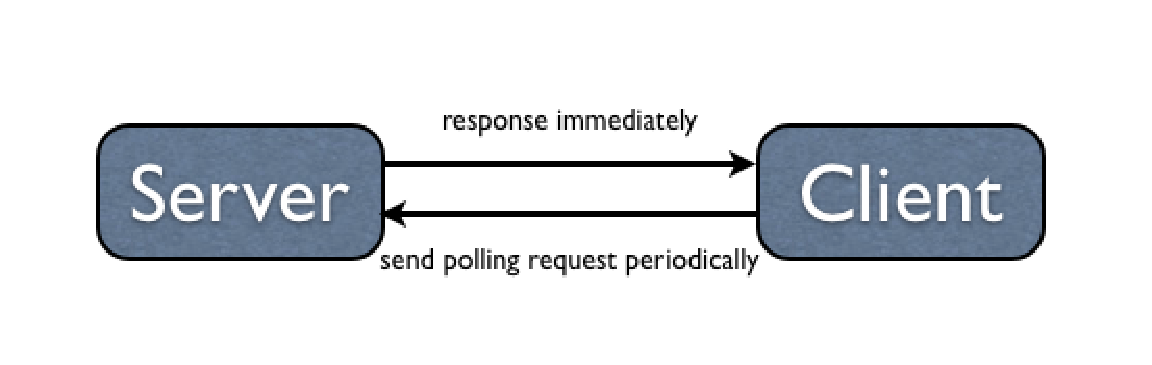
\includegraphics[scale=0.45]{figures/client_poll.eps}
    \caption{Twisted Event Loop}
    \label{fig:Client Polling}
\end{figure}

\subsection{Design Goals and Rationale\\}

\begin{itemize}
\item {\bf Scalability}  
    As the long polling technologies requires the server to keep the polliing request active for a period of time,
    large number of concurrent clients will generate lots of active connections. One of our goal is to minimize the 
    cost of maintaining these active connections, which could in turn enhance the system's scalability.
     
    Scalability is the main issue in a Push model. Web servers usually create a thread per
    client (connection). However, an HTTP based push will have an
    outstanding request waiting on the server which will be used to send a response to the
    client the instant an asynchronous event occurs. 
    
    However, for the http-based polling request, a large portion of the time will spent in waiting for new events, which
    makes the traditonal multi-thread model inefficient. Better technologies are needed 

\item {\bf Transparancy} TODO: many backend are implement in multi-thread model, so ... be able to have the long polling service with minimal effort (with little modification of the original service).

\item {\bf Low latency} TODO: overhead is inevitable, how to minimize it?

\item {\bf Generality} TODO: can be used in many scenarios.

\end{itemize}

\subsection{System Overview\\}

TODO: a figure to illustrate the main idea.

\begin{figure}[htb!]
\centering%
    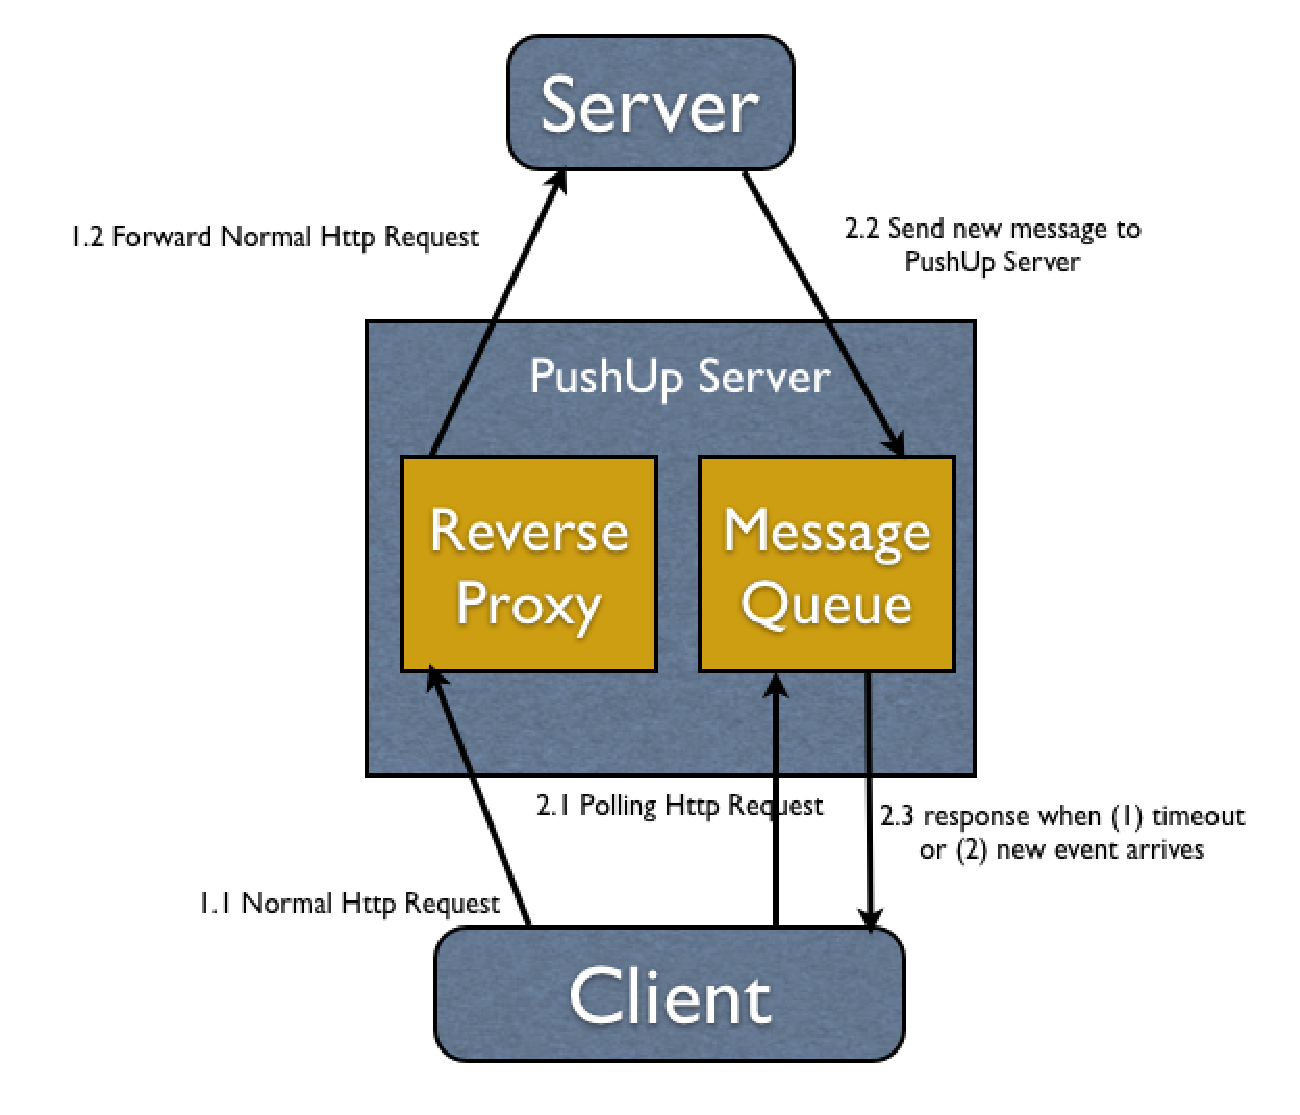
\includegraphics[scale=0.40]{figures/simple_pushup_arch.eps}
    \caption{Simplified PushUp Architecture}
    \label{fig:eventloop}
\end{figure}

TODO: Overall description of such design. and how it matches the rationale mentioned above.


\subsection{Reverse Proxy\\}

Why reverse proxy

How it works. Briefly

\subsection{Message Queue\\}

Why Message Queue, 

How it works, briefly


